\documentclass[conference]{IEEEtran}
% \IEEEoverridecommandlockouts
% The preceding line is only needed to identify funding in the first footnote. If that is unneeded, please comment it out.
\usepackage{cite}
\usepackage{amsmath,amssymb,amsfonts}
\usepackage{algorithmic}
\usepackage{graphicx}
\usepackage{textcomp}
\usepackage{xcolor}
\usepackage{booktabs}
\usepackage{multirow}
\usepackage{enumitem}
\usepackage{url}
\usepackage{tabularx}
\usepackage{hyperref}

\bibliographystyle{IEEEtran}

\def\BibTeX{{\rm B\kern-.05em{\sc i\kern-.025em b}\kern-.08em
    T\kern-.1667em\lower.7ex\hbox{E}\kern-.125emX}}
\begin{document}


\title{\textit{Systematic Capability Benchmarking of Frontier Large Language Models for Offensive Cyber Tasks}
% \thanks{Identify applicable funding agency here. If none, delete this.}
}

%\author{\IEEEauthorblockN{Anonymous Authors}}
% \author{%
%   \IEEEauthorblockN{%
%     Tyler H. Merves\IEEEauthorrefmark{1},
%     Michael H. Conaway\IEEEauthorrefmark{1},
%     Joseph M. Escobar\IEEEauthorrefmark{1}, 
%     Hakan T. Otal\IEEEauthorrefmark{2}, and
%     Unal Tatar\IEEEauthorrefmark{1}
%   }%
% \IEEEauthorblockA{ \IEEEauthorrefmark{1} Department of Cybersecurity \\ \IEEEauthorrefmark{2} Department of Information Sciences and Technology\\ College of Emergency Preparedness, Homeland Security, and Cybersecurity \\ \textit{University at Albany, SUNY, USA}\\ \textit{ tmerves, mhconaway, jmescobar, hotal, utatar [at] albany [dot] edu}}%

%  % \vspace{-4.6mm}
% }

\author{ 
    \fontsize{10}{12}\selectfont
    Tyler H. Merves\textsuperscript{1},
    Michael H. Conaway\textsuperscript{1},
    Joseph M. Escobar\textsuperscript{1}, 
    Hakan T. Otal\textsuperscript{2},
    and Unal Tatar\textsuperscript{1} \\        
    *\textit{tmerves, mhconaway, jmescobar, hotal, utatar [at] albany [dot] edu} \\ \\
    
    \begin{tabularx}{\textwidth}{>{\centering\arraybackslash}X}
        \fontsize{9}{10}\selectfont \textsuperscript{1} \textit{Department of Cybersecurity}  & 
        \fontsize{9}{10}\selectfont \textsuperscript{2} \textit{Department of Information Sciences and Technology} \\ 
        \fontsize{9}{10}\selectfont \textit{College of Emergency Preparedness, Homeland Security, and Cybersecurity} \\
        \fontsize{9}{10}\selectfont \textit{University at Albany, SUNY} \\
        \fontsize{9}{10}\selectfont \textit{Albany, NY, USA}
    \end{tabularx}
}

\maketitle

\begin{abstract}
ABSTRACT WILL BE WRITTEN AT THE END OF THE PAPER
\end{abstract}

\begin{IEEEkeywords}
large language models, capture the flag, cybersecurity benchmarking, multi-agent systems, penetration testing, LLM evaluation, offensive security
\end{IEEEkeywords}

\section{Introduction}

\noindent\textbf{Motivation \& Context:}
\begin{itemize}
  \item LLMs are demonstrating growing capability in cybersecurity tasks (vulnerability discovery, exploit generation, penetration testing).
  \item Capture The Flag (CTF) competitions serve as standardized proxies for measuring offensive cyber capability.
  \item Recent work (D-CIPHER, NYU CTF Bench, EnIGMA, CRAKEN) has shown multi-agent LLM architectures can solve CTF challenges, but comparisons across models and configurations remain fragmented.
  \item No prior study systematically varies environment, prompts, model selection, and architecture on the same benchmark.
\end{itemize}

\noindent\textbf{Problem Statement:}
\begin{itemize}
  \item It is unclear which frontier LLMs perform best on offensive cyber tasks, what environmental tooling matters, and how reliable reported results are given LLM non-determinism.
\end{itemize}

\noindent\textbf{Contributions:}
\begin{enumerate}
  \item First systematic comparison of 10 frontier LLMs (from 7 providers) on 200 CTF challenges using a unified multi-agent framework.
  \item $2\!\times\!2\!\times\!2$ factorial analysis of environment (Ubuntu/Kali), prompt strategy (generic/tips), and auto-prompting, providing evidence that Kali Linux provides +9.5\,pp improvement while auto-prompting hurts.
  \item Cost-performance analysis revealing Gemini 3 Flash achieves 8.6$\times$ better cost-efficiency than Gemini 3 Pro.
  % \item Reproducibility study showing dramatic run-to-run variance (13.5\%--52\%), highlighting a methodological gap in LLM benchmarking.
  \item Open experimental infrastructure: Kali Docker image, tool documentation lookup agents, parallel experiment runner, result parsing/visualization pipeline.
\end{enumerate}


\section{Methodology}

We extend the D-CIPHER multi-agent framework with new backends, environments, and tooling, then conduct a systematic evaluation across four research questions on the NYU CTF Bench.

\subsection{D-CIPHER Framework}

\begin{itemize}
  \item D-CIPHER is a multi-agent Planner--Executor architecture for solving CTF challenges~\cite{dcipher}... 
\end{itemize}
\noindent\textbf{Extensions to D-CIPHER:}
\begin{itemize}
  \item Added Vertex AI, OpenRouter, and Ollama backends to support 9+ model providers beyond the original OpenAI-only setup.
  \item Added \texttt{LookupCommandTool} and \texttt{ListCommandsTool} so the agent can query Kali tool documentation at runtime.
\end{itemize}

% TODO: Add architecture diagram showing Planner -> Executor -> Docker container flow, with optional AutoPrompter.

\subsection{Benchmark Dataset}

\begin{itemize}
  \item NYU CTF Bench~\cite{nyuctfbench}: 200 challenges from real CTF competitions, spanning 6 categories.
  \item Category distribution: crypto~(52), reverse~(51), pwn~(39), misc~(24), web~(19), forensics~(15).
  \item Challenges range from beginner to advanced difficulty across competitions from 2016--2024.
  \item Each challenge includes source files, a Docker environment, and a ground-truth flag for automated verification.
\end{itemize}

% TODO: Add table: category breakdown (category, count, example techniques required).

\subsection{Experimental Design}

\begin{itemize}
  \item We address four research questions through controlled experiments on the full 200-challenge set using D-CIPHER with Gemini 3 Pro (via Vertex AI) as the default model.
  \item \textbf{Metrics:} solve rate (solved\,/\,200), total API cost, cost per solved challenge, exit reason distribution, and per-category solve rates.
\end{itemize}

\subsubsection{RQ1 \& RQ2: Environment and Prompt Engineering}

\begin{itemize}
  \item $2\!\times\!2\!\times\!2$ factorial design: Environment (Ubuntu~22.04 vs.\ Kali Linux) $\times$ Prompts (Generic vs.\ Category-specific tips) $\times$ AutoPrompt (Off vs.\ On).
  \item 8 total conditions, each run on all 200 challenges with Gemini 3 Pro.
  \item \textbf{Ubuntu} = base Docker image with standard tools (gdb, radare2, pwntools, angr, etc.).
  \item \textbf{Kali} = custom Docker image with 100+ pre-installed penetration testing tools + \texttt{commands\_documentation.csv} for agent lookup.
  \item \textbf{Generic prompts} = minimal instructions; \textbf{Tips prompts} = category-specific guidance (e.g., ``Use pwntools for binary exploitation'').
  \item \textbf{AutoPrompt} = agent explores challenge files first and generates a tailored prompt before solving.
\end{itemize}

\subsubsection{RQ3: Model Selection}

\begin{itemize}
  \item 10 models benchmarked from 7 providers, all using Kali + generic prompts (best RQ1/RQ2 condition).
  \item Models: Claude 4.5 Opus (Anthropic); Gemini 3 Pro, Gemini 3 Flash (Google); GPT-5.2, GPT-5.2-Codex (OpenAI); GLM-5 (Z-AI); DeepSeek-R1, DeepSeek-V3 (DeepSeek); Llama 3.3 70B (Meta); Qwen 3.5 397B-A17B (Alibaba).
  \item Model types span: frontier, small/efficient, reasoning, code-specialized, open-source.
  \item All models use identical configuration (max rounds, temperature, toolset) to ensure fair comparison.
\end{itemize}

\subsubsection{RQ4: Multi-Agent Architecture}

\begin{itemize}
  \item Test whether asymmetric Planner/Executor model assignment improves cost-performance.
  \item 4 conditions: Gemini 3 Pro (both), Gemini 3 Flash (both), Pro Planner + Flash Executor, and Flash Planner + Pro Executor.
  \item Hypothesis: strong planner + cheap executor achieves near-Pro accuracy at near-Flash cost.
\end{itemize}

% \subsubsection{RQ5: Reproducibility}
% 
% \begin{itemize}
%   \item 4 identical runs of Gemini 3 Pro + Kali + Generic to quantify run-to-run variance.
%   \item Temperature $= 1.0$ (following D-CIPHER paper recommendation for optimal performance).
%   \item Measures: solve rate, per-category variance, cost variance.
% \end{itemize}


\section{Experimental Results}

We present results for each of the four research questions on the full 200-challenge NYU CTF Bench.

\subsection{RQ1 \& RQ2: Impact of Environment and Prompt Strategy}

Figure~\ref{fig:rq12_heatmap} summarizes the $2\!\times\!2\!\times\!2$ factorial results (Environment $\times$ Prompts $\times$ AutoPrompt), all run with Gemini~3~Pro.

% \noindent\textbf{Environment effect (RQ1).}
Kali Linux consistently outperforms Ubuntu in matched conditions. Under identical prompt settings (Generic, no AutoPrompt), Kali achieves 52.0\% (104/200) versus 42.5\% (85/200) for Ubuntu, a gain of $+9.5$\,pp. The advantage is especially pronounced in forensics ($46.7\%$ vs.\ $20.0\%$) and reverse engineering ($58.8\%$ vs.\ $49.0\%$), categories that depend heavily on specialized tool availability. The Kali Docker image ships with over 100 pre-installed penetration-testing tools and a structured documentation file that agents can query at runtime, reducing tool-discovery friction.

% \noindent\textbf{Prompt strategy effect (RQ2).}
The interaction between environment and prompt strategy is noteworthy. Under Kali, generic prompts outperform category-specific tips ($52.0\%$ vs.\ $40.0\%$), whereas under Ubuntu the pattern reverses ($42.5\%$ vs.\ $44.5\%$). A likely explanation is that the richly tooled Kali environment already encodes implicit guidance; layering explicit tips over-constrains the agent's exploration. On Ubuntu, the sparser environment means tips compensate by steering the agent toward appropriate techniques.

% \noindent\textbf{AutoPrompt effect.}
Auto-prompting, in which the agent explores challenge files and generates a tailored prompt before solving, generally \emph{hurts} performance. Under Kali + Generic, AutoPrompt reduces the solve rate from $52.0\%$ to $39.5\%$ ($-12.5$\,pp); under Ubuntu + Tips, the drop is even sharper: $44.5\%$ to $16.0\%$ ($-28.5$\,pp). One exception stands out: under Kali + Tips, AutoPrompt raises the rate from $40.0\%$ to $48.5\%$ ($+8.5$\,pp), suggesting it can partially recover a sub-optimal base strategy. We hypothesize that the additional exploration phase typically consumes budget without producing actionable insight, and may introduce misleading preliminary analysis.

The best overall configuration (Kali + Generic without AutoPrompt) costs \$44.23 total. Notably, the most expensive configuration (Kali + Tips + AutoPrompt, \$66.12) achieves only the second-best solve rate (48.5\%), reinforcing that simpler configurations dominate.

\begin{figure*}[t]
  \centering
  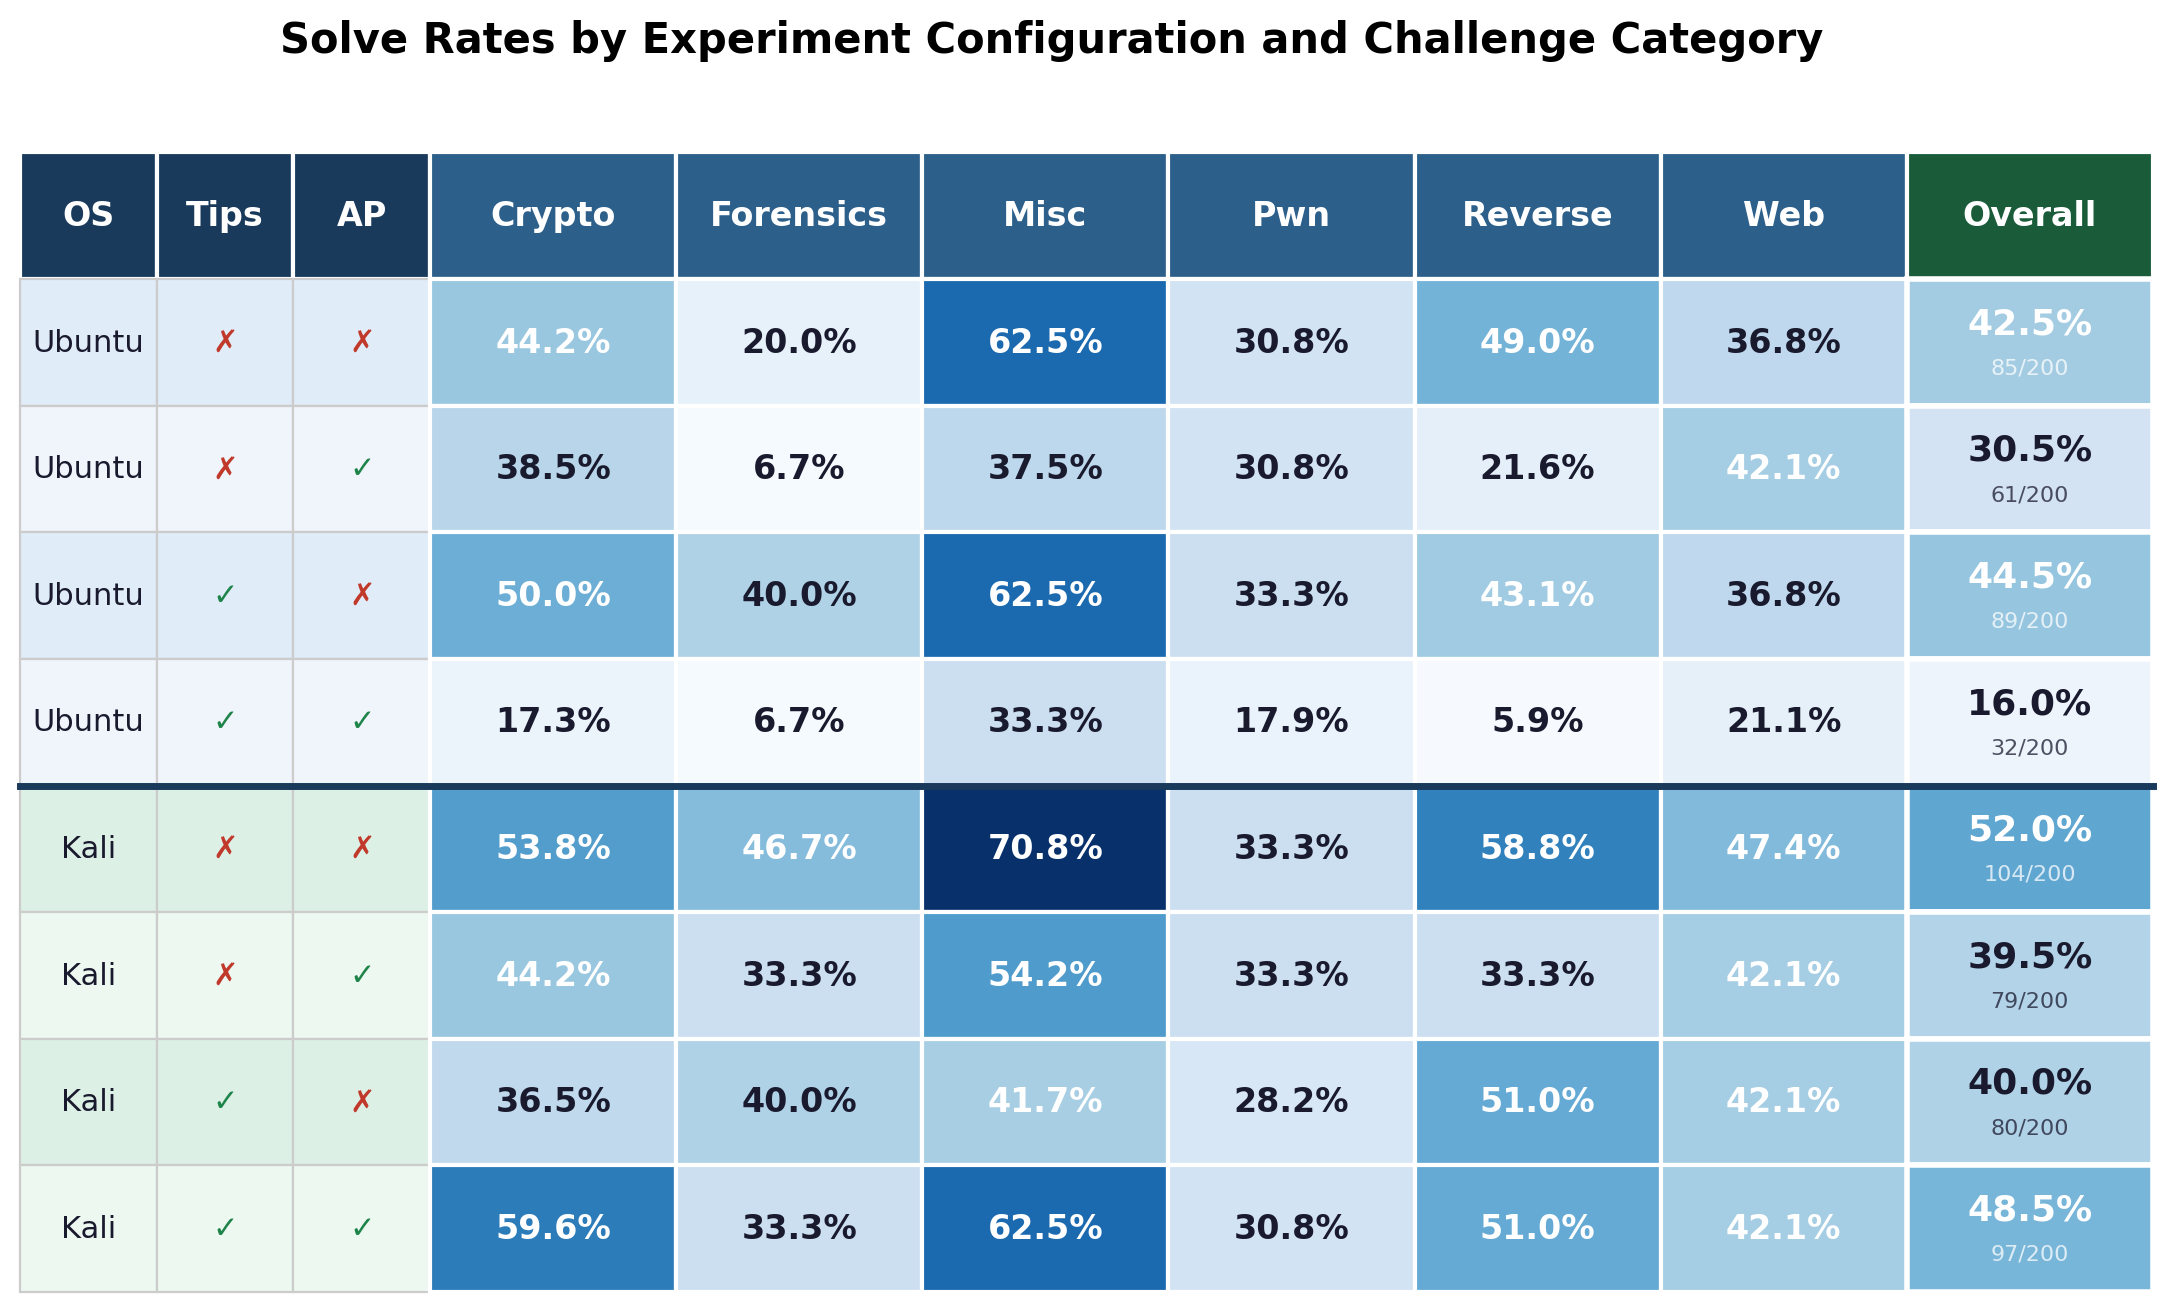
\includegraphics[width=0.6\linewidth]{./figures/rq1rq2_heatmap_table.png}
  \caption{Solve rates by configuration and challenge category (RQ1+RQ2).}
  \label{fig:rq12_heatmap}
\end{figure*}

\subsection{RQ3: Model Selection}

We benchmark ten frontier LLMs from seven providers under the best RQ1/RQ2 configuration (Kali + Generic, no AutoPrompt). Table~\ref{tab:rq3_results} reports solve rates, total costs, and cost-per-solve; Figure~\ref{fig:rq3_cost} visualizes the cost--performance tradeoff.

\begin{table}[t]
\centering
\caption{Model benchmark on NYU CTF Bench \\(200 Challenges on Kali with Generic prompts)}
\label{tab:rq3_results}
\footnotesize
\begin{tabular}{@{}llrrrr@{}}
\toprule
\textbf{Model} & \textbf{Provider} & \textbf{Solved} & \textbf{Rate} & \textbf{Cost (\$)} \\ % & \textbf{\$/Solve} \\
\midrule
Claude 4.5 Opus    & Anthropic & 118 & \%59.0 & \$18.57 \\
Gemini 3 Pro       & Google    & 104 & \%52.0 & \$44.23 \\
Gemini 3 Flash     & Google    &  54 & \%27.0 &  \$2.69 \\
GLM-5              & Z-AI      &  39 & \%19.5 & \$22.09 \\
GPT-5.2-Codex      & OpenAI    &  36 & \%18.0 &  \$9.23 \\
GPT-5.2            & OpenAI    &  27 & \%13.5 &  \$7.47 \\
DeepSeek-V3        & DeepSeek  &  13 &  \%6.5 &  \$0.19 \\
DeepSeek-R1        & DeepSeek  &   8 &  \%4.0 &  \$0.13 \\
Qwen-3.5-397B-A17B & Alibaba   &   7 &  \%3.5 &  \$1.39 \\
Llama-3.3-70B      & Meta      &   5 &  \%2.5 &  \$0.03 \\
\bottomrule
\end{tabular}
\end{table}

% \noindent\textbf{Overall ranking and provider hierarchy.}
Claude~4.5~Opus leads at 59.0\% (118/200), followed by Gemini~3~Pro at 52.0\% (104/200). These two models form a clear top tier, each solving at least $1.9\times$ more challenges than the third-ranked Gemini~3~Flash (27.0\%). OpenAI's models cluster in the middle tier: GPT-5.2-Codex (18.0\%) outperforms base GPT-5.2 (13.5\%), suggesting code specialization provides a meaningful advantage. Z-AI's GLM-5 (19.5\%) achieves competitive accuracy but at disproportionate cost (\$0.57/solve). Open-source models (Llama~3.3~70B, Qwen~3.5) and DeepSeek variants perform poorly at 2.5--6.5\%, likely due to weaker tool-use and multi-turn agentic reasoning capabilities.

% \noindent\textbf{Reasoning vs.\ agentic capability.}
The DeepSeek pair provides an instructive comparison: the reasoning-specialized R1 (4.0\%) does \emph{not} outperform the standard V3 (6.5\%). This suggests that in agentic settings, where success depends on iterative tool calls and multi-step environment interaction, robust tool-use matters more than pure chain-of-thought reasoning.

% \noindent\textbf{Failure modes.}
Failure patterns vary qualitatively across models. DeepSeek models fail predominantly by timeout (188/200 for R1), indicating inability to make progress. GPT-5.2 exhibits a high error rate (88/200), suggesting tool-framework integration issues. Llama~3.3~70B prematurely gives up on 160/200 challenges. In contrast, Gemini~3~Pro fails more gracefully, hitting cost (30) or round (41) limits, indicating productive progress that simply exhausts the budget. Claude~4.5~Opus shows 75 error exits among its 82 unsolved challenges; when these integration issues are absent, the model performs strongly.

% \noindent\textbf{Category patterns.}
The \textit{misc} category is the easiest across nearly all models, while \textit{pwn} is consistently the hardest. Claude~4.5~Opus outperforms Gemini~3~Pro in every category, with the largest gains in pwn (41.0\% vs.\ 33.3\%) and web (52.6\% vs.\ 47.4\%).

% \noindent\textbf{Cost-efficiency.}
Gemini~3~Flash occupies a uniquely favorable position on the cost--performance frontier (Figure~\ref{fig:rq3_cost}): at \$0.05/solve, it is $8.6\times$ cheaper than Gemini~3~Pro and $3.2\times$ cheaper than Claude~4.5~Opus, while solving over half of what Pro achieves at 6\% of the cost. Claude~4.5~Opus, despite its highest absolute accuracy, is more cost-effective than Gemini~3~Pro (\$0.16 vs.\ \$0.43 per solve) due to lower total cost and higher solve count.

\begin{figure}[t]
  \centering
  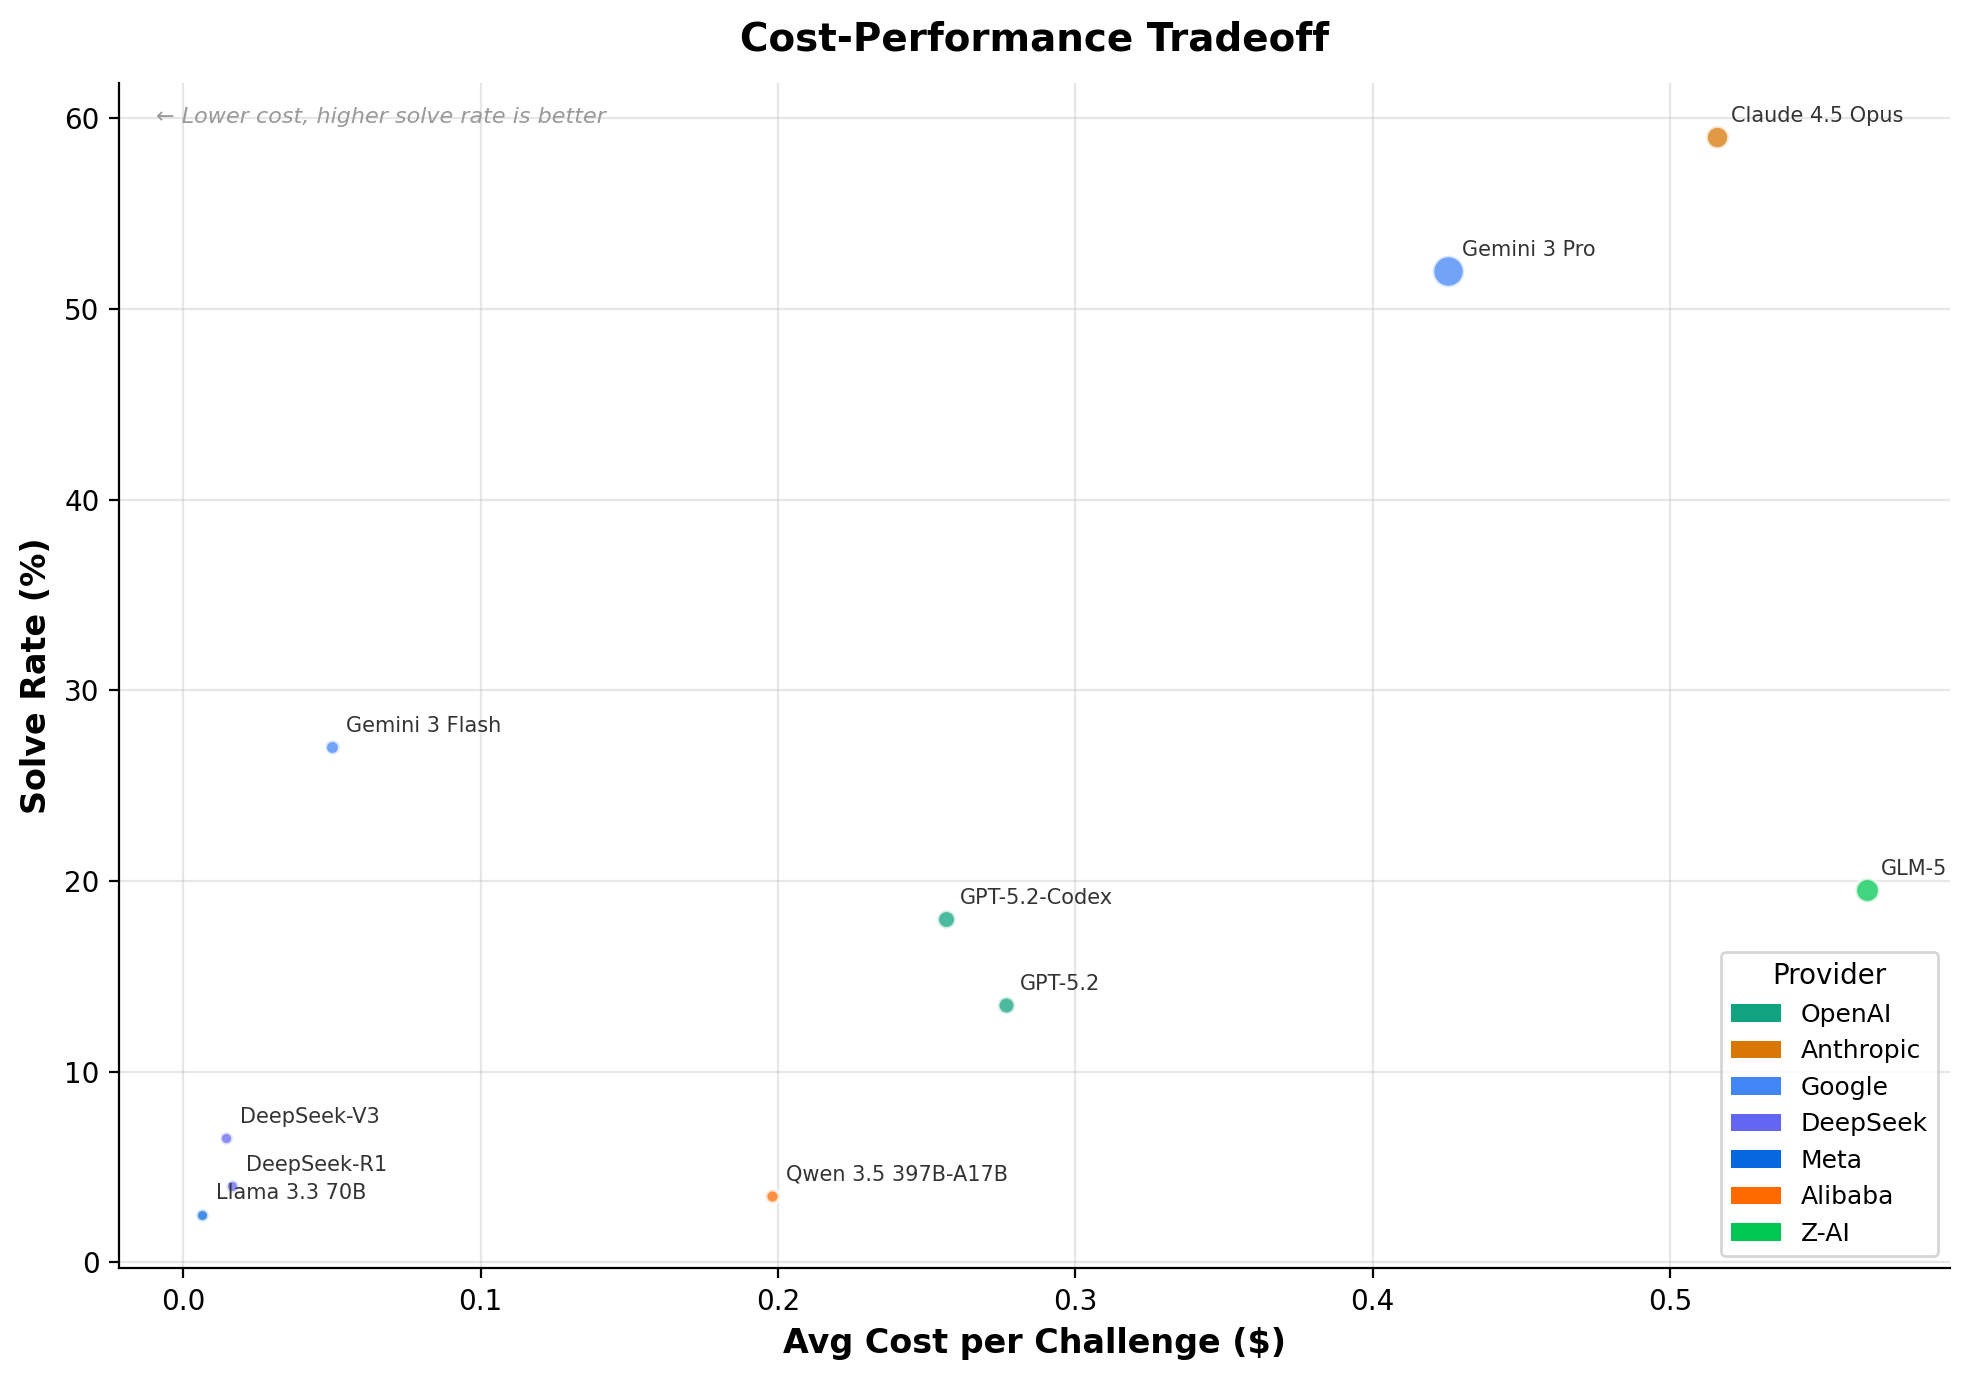
\includegraphics[width=\columnwidth]{./figures/rq3_cost_vs_solve.png}
  \caption{Cost--performance tradeoff: average cost per challenge vs.\ solve rate. Bubble size is proportional to total cost. The upper-left region is optimal.}
  \label{fig:rq3_cost}
\end{figure}

\subsection{RQ4: Multi-Agent Architecture}

Table~\ref{tab:rq4_results} presents results for four planner/executor configurations using Gemini~3~Pro and Flash, all under Kali + Generic.

\begin{table}[t]
\centering
\caption{Planner/Executor architecture comparison \\(200 challenges, Kali + Generic).}
\label{tab:rq4_results}
\footnotesize
\begin{tabular}{@{}llrrr@{}}
\toprule
\textbf{Planner} & \textbf{Executor} & \textbf{Solved} & \textbf{Rate} & \textbf{Cost (\$)} \\
\midrule
Pro   & Pro   & 104 & 52.0\% & 44.23 \\
Pro   & Flash &  57 & 28.5\% &  3.90 \\
Flash & Flash &  54 & 27.0\% &  2.69 \\
Flash & Pro   &  47 & 23.5\% &  2.92 \\
\bottomrule
\end{tabular}
\end{table}

The homogeneous Pro configuration achieves 52.0\%, nearly doubling the next-best result. The asymmetric Pro~Planner + Flash~Executor yields only $+1.5$\,pp over Flash-only (28.5\% vs.\ 27.0\%) while increasing cost by 45\%, a poor tradeoff.

Most surprisingly, the reverse configuration (Flash~Planner + Pro~Executor) performs \emph{worse} than Flash-only (23.5\% vs.\ 27.0\%), despite deploying the stronger model as executor. This challenges the intuition that executor quality is the bottleneck; instead, it suggests that \emph{coherent planning and execution within the same model} matters more than the raw capability of either role alone. The performance gap is largest in categories requiring sustained multi-step reasoning: crypto (53.8\% for Pro-only vs.\ 21.1\% for Pro+Flash) and misc (70.8\% vs.\ 29.2\%). The practical implication is clear: invest in the best model for \emph{both} roles rather than optimizing with mixed tiers.

% \subsection{RQ5: Reproducibility}
% 
% To quantify run-to-run variance, we execute four identical runs of the best configuration (Gemini~3~Pro, Kali, Generic, $T{=}1.0$). Figure~\ref{fig:rq5_repro} displays the results.
% 
% The four runs yield solve rates of 52.0\%, 22.5\%, 26.0\%, and 13.5\% ($\mu = 28.5\%$, $\sigma = 14.3\%$). The best run solves $3.9\times$ more challenges than the worst under \emph{identical} settings. Total costs range from \$3.68 to \$44.23, an order-of-magnitude spread. Per-category analysis confirms this instability is pervasive: no single category drives the variance, with the widest spreads in misc (16.7\%--70.8\%), reverse (21.6\%--58.8\%), and crypto (17.3\%--53.8\%).
% 
% These findings carry significant methodological implications. Run~1, taken in isolation, would characterize Gemini~3~Pro as solving over half of all challenges; Run~4 would label it a weak performer at 13.5\%. Single-run benchmarks, as commonly reported, may substantially misrepresent true capability. We argue that the field requires standardized reproducibility protocols: results should report multiple replications with confidence intervals, and cross-model comparisons are meaningful only when evaluated across the same number of trials.
% 
% \begin{figure}[t]
%   \centering
%   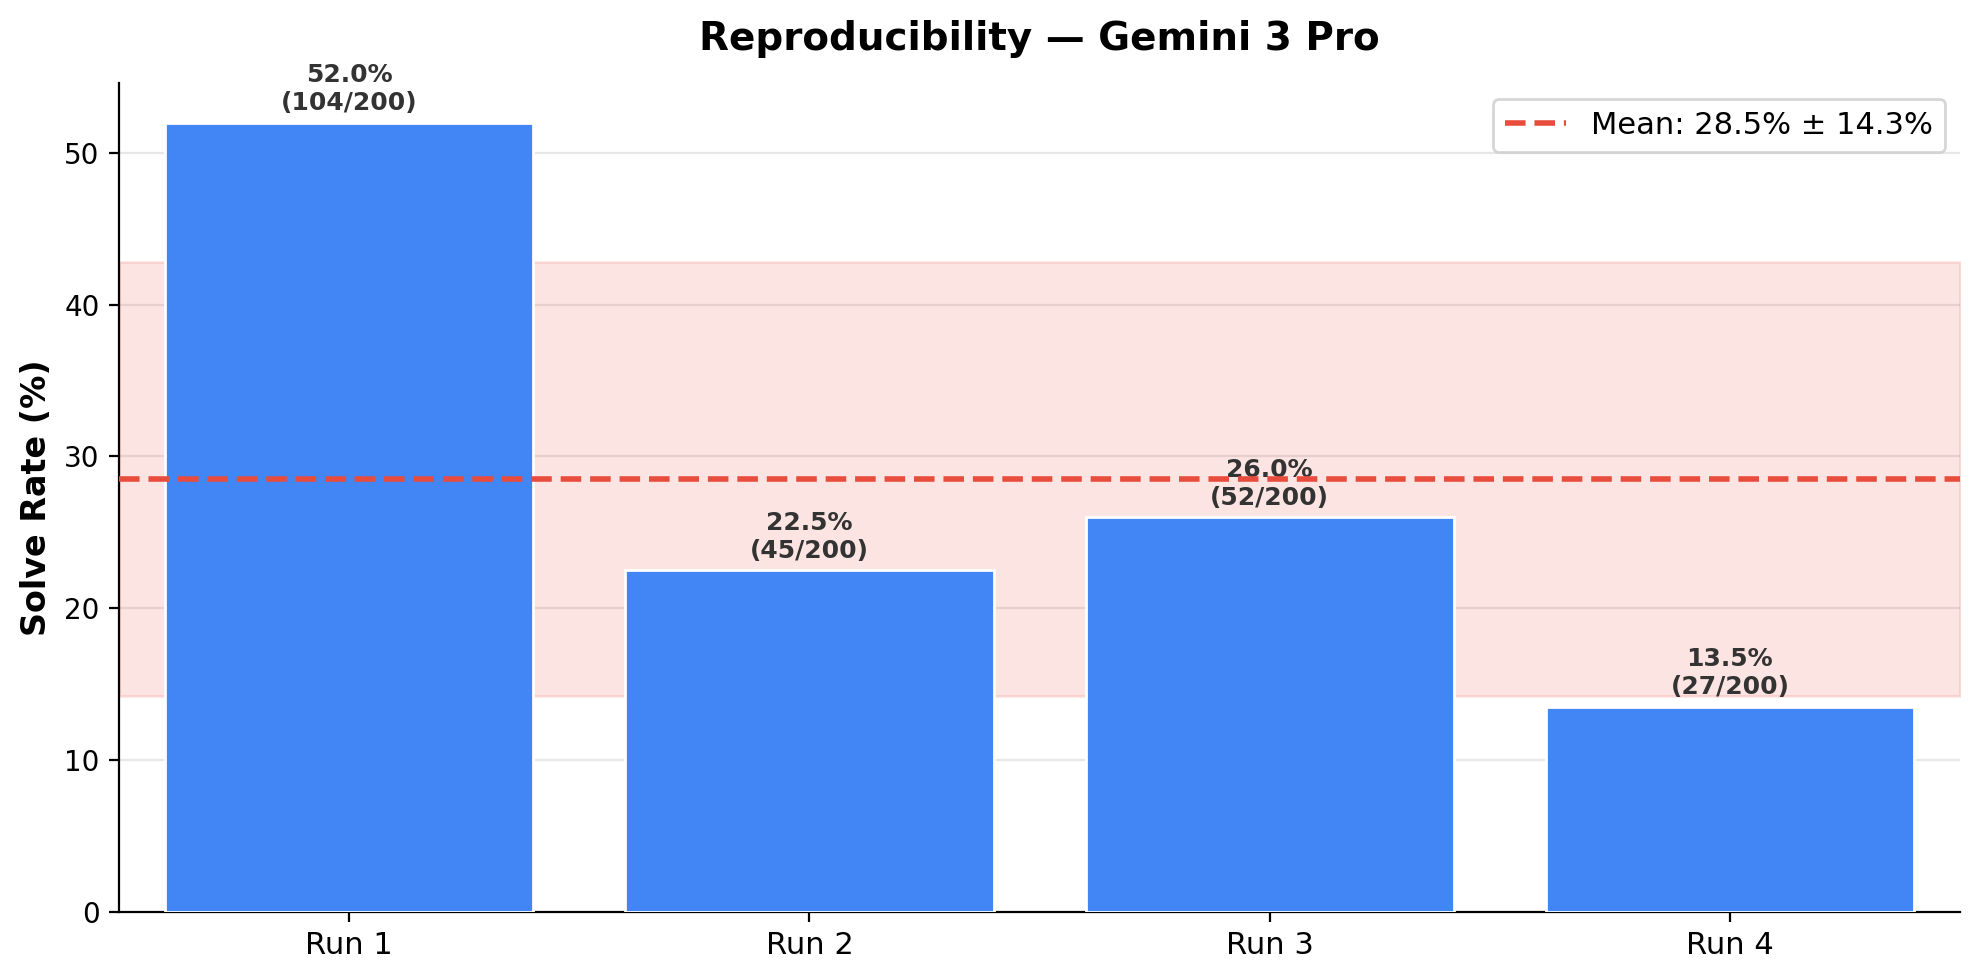
\includegraphics[width=\columnwidth]{./figures/rq5_reproducibility.png}
%   \caption{Reproducibility: solve rates across four identical runs of Gemini~3~Pro. Dashed line shows the mean ($28.5\%$); shaded band indicates $\pm 1\sigma$ ($14.3\%$).}
%   \label{fig:rq5_repro}
% \end{figure}


\section{Conclusion}

\noindent\textbf{Summary:}
\begin{itemize}
  \item We benchmarked 10 frontier LLMs on 200 CTF challenges. Claude 4.5 Opus achieves the highest solve rate at 59\%, while Gemini 3 Flash offers $8.6\times$ better cost-efficiency at \$0.05/solve.
  \item Kali Linux provides +9.5\,pp over Ubuntu; auto-prompting and specialized tips generally hurt performance, and simpler configurations work best.
  \item Asymmetric planner/executor architectures do not yield meaningful cost-performance benefits; coherent same-model configurations outperform mixed-tier pairings.
  % \item Run-to-run variance (13.5--52\%) is alarmingly high, challenging single-run benchmarks. Results should include multiple runs with confidence intervals.
\end{itemize}

\noindent\textbf{Limitations:}
\begin{itemize}
  \item Results are specific to D-CIPHER; other frameworks may show different patterns.
  \item NYU CTF Bench skews toward academic CTF styles; model rankings reflect early-2026 versions and may shift.
\end{itemize}

\noindent\textbf{Future Work:}
\begin{itemize}
  \item Expand to CyBench (90 challenges) for cross-benchmark validation; test RAG pipelines and adaptive difficulty routing.
  \item Investigate why pwn/forensics remain difficult across all models; develop standardized reproducibility protocols for LLM benchmarking.
\end{itemize}


\section*{Acknowledgment}

This research was supported by the SUNY AI Platform, powered by Google Cloud, which provided Vertex AI and compute infrastructure for large-scale LLM benchmarking.

VICEROY ?

\nocite{*}
 % \vspace{-2mm}
\bibliography{paper}

\end{document}
